%!TEX TS-program = xelatex

\documentclass[t]{beamer}

\usetheme{Hannover}
\usecolortheme{rose}

%%% Работа с русским языком
\usepackage[english,russian]{babel}   %% загружает пакет многоязыковой вёрстки
\usepackage{fontspec,xltxtra,xunicode}      %% подготавливает загрузку шрифтов Open Type, True Type и др.
%\defaultfontfeatures{Ligatures={TeX},Renderer=Basic}  %% свойства шрифтов по умолчанию
\setmainfont[Ligatures={TeX,Historic},
SmallCapsFont={Brill},
SmallCapsFeatures={Letters=SmallCaps}]{Brill} %% задаёт основной шрифт документа
\setsansfont{Brill}                    %% задаёт шрифт без засечек
\setmonofont[Ligatures=NoCommon]{DejaVu Sans}
\newfontfamily\SYM{Brill}
\usepackage{indentfirst}
%%% Дополнительная работа с математикой
\usepackage{amsmath,amsfonts,amssymb,amsthm,mathtools} % AMS
\usepackage{icomma} % "Умная" запятая: $0,2$ --- число, $0, 2$ --- перечисление

%%% Работа с картинками
\usepackage{wrapfig} % Обтекание рисунков текстом
\usepackage{rotating}
\usepackage{fixltx2e}
\usepackage{hhline}
\usepackage{lscape}

%%% Работа с таблицами
\usepackage{array,tabularx,tabulary,booktabs} % Дополнительная работа с таблицами
\usepackage{longtable}  % Длинные таблицы
\usepackage{multirow} % Слияние строк в таблице

\usepackage{multicol} % Несколько колонок
%%% Страница
%\usepackage{fancyhdr} % Колонтитулы
% 	\pagestyle{fancy}
 	%\renewcommand{\headrulewidth}{0pt}  % Толщина линейки, отчеркивающей верхний колонтитул
% 	\lfoot{Нижний левый}
% 	\rfoot{Нижний правый}
% 	\rhead{Верхний правый}
% 	\chead{Верхний в центре}
% 	\lhead{Верхний левый}
%	\cfoot{Нижний в центре} % По умолчанию здесь номер страницы

\usepackage{setspace} % Интерлиньяж
%\onehalfspacing % Интерлиньяж 1.5
%\doublespacing % Интерлиньяж 2
\singlespacing % Интерлиньяж 1

\usepackage{subfig} % подкартинки
\usepackage{lastpage} % Узнать, сколько всего страниц в документе.
\usepackage{soul} % Модификаторы начертания
\usepackage{bbding}
\usepackage{tikz} % Работа с графикой
\usepackage{pgfplots}
\usepackage{pgfplotstable}
\usepackage{verbatim}

\usepackage{attachfile2}
\usepackage{alltt}

%%% Лингвистические пакеты
%\usepackage{savetrees} % пакет, который экономит место
\usepackage{forest} % для рисования деревьев
\usepackage{vowel} % для рисования трапеций гласных
\usepackage{natbib}
\bibpunct[: ]{[}{]}{;}{a}{}{,}
\usepackage[nogroupskip,nopostdot, nonumberlist]{glossaries}
%\usepackage{glossary-mcols} 
%\setglossarystyle{mcolindex}
\usepackage{philex} % пакет для примеров
\newcommand{\mytem}{\item[$\circ$]}
\addto\captionsrussian{
\renewcommand{\refname}{}}

\newcommand{\apostrophe}{\XeTeXglyph\XeTeXcharglyph"0027\relax}
\usetikzlibrary{patterns}

\usepackage{ulem}

\usepackage{hyperref}
\hypersetup{ % Гиперссылки
	colorlinks=true, % false: ссылки в рамках; true: цветные ссылки
	linkcolor=black, % внутренние ссылки
	citecolor=black, % на библиографию
	filecolor=black, % на файлы
	urlcolor=blue % на URL
	}
\setbeamercolor{alerted text}{fg=blue}
\setbeamersize{text margin left=4mm,text margin right=1mm} 
\setbeamertemplate{frametitle}[default][center]
\setbeamertemplate{navigation symbols}{
	\usebeamerfont{footline}%
    \usebeamercolor[fg]{footline}%
    \hspace{1em}%
    {{\small презентация доступна: \href{https://bit.ly/2NT0OUN}{\textbf{bit.ly/2NT0OUN}}}
    \hspace{5cm}
    \insertframenumber/\inserttotalframenumber\vspace{0.5mm}}}
\title[]{Акустическая фонетика за 90 минут}
\author[]{Г. Мороз}
\date{30 июля, 2018}
\begin{document}
\frame{\titlepage}
\section{мифы}
\begin{frame}{Список мифов, чтобы мы были на одной волне:}
\begin{itemize}
\item люди отличаются от животных своей способностью мыслить и коммуницировать (по другой версии --- шутить и смеяться) \pause
\begin{itemize}
\item животные много общаются и передают друг другу информацию \pause
\item животные способны мыслить \pause
\item животные на каком-то уровне могут выучить человеческие языки \pause
\end{itemize}
\item люди общаются при помощи слов и речи \pause
\begin{itemize}
\item контекст, мимика, жесты говорят порой больше, чем слова \pause
\item люди, слава богу, научились писать \pause
\item бывают жестовые языки
\end{itemize}
\item хорошее распознавание лучше сделает программист, а не лингвист\pause . К сожалению, это не миф...
\end{itemize}
\end{frame}
\section{классификация звуков}
\begin{frame}{Классификация звуков:  способ образования}
\begin{itemize}
\item гласные: и, у, я...
\item согласные
\begin{itemize}
\item сонорные
\begin{itemize}
\item носовые: м, н
\item плавные: л, р
\item глайды: й, w
\end{itemize}
\item шумные
\begin{itemize}
\item взрывные: п, т, к
\item фрикативные: с, ш, х
\item аффрикаты: ц, ч, ть
\end{itemize}
\end{itemize}
\end{itemize}
\end{frame}


\begin{frame}{Классификация звуков:  место образования}

\end{frame}

\section{гласные}
\begin{frame}{Как форма речевого аппарата влияет на гласные?}
\Large
\vfill
\begin{center}
\begin{vowel}
\putcvowel[l]{i}{1}
\putcvowel[r]{y}{1}
\putcvowel[l]{e}{2}
\putcvowel[r]{ø}{2}
\putcvowel[l]{ɛ}{3}
\putcvowel[r]{œ}{3}
\putcvowel[l]{a}{4}
\putcvowel[r]{ɶ}{4}
\putcvowel[l]{ɑ}{5}
\putcvowel[r]{ɒ}{5}
\putcvowel[l]{ʌ}{6}
\putcvowel[r]{ɔ}{6}
\putcvowel[l]{ɤ}{7}
\putcvowel[r]{o}{7}
\putcvowel[r]{u}{8}
\putcvowel[l]{ɯ}{8}
\putcvowel[r]{ɨ}{9}
\putcvowel[l]{ʉ}{9}
\putcvowel[r]{ɘ}{10}
\putcvowel[l]{ɵ}{10}
\putcvowel{ə}{11}
\putcvowel[r]{ɜ}{12}
\putcvowel[l]{ɞ}{12}
\putcvowel{ɪ ʏ}{13}
\putcvowel{ʊ}{14}
\putcvowel{ɐ}{15}
\putcvowel{æ}{16}
\end{vowel}
\end{center}
\vfill
\normalsize
Исторически подъем и ряд --- импрессионистические лингвистические понятия.
\end{frame}

\begin{frame}{Как форма речевого аппарата влияет на гласные?}
\Large
\vfill
\begin{center}
\begin{vowel}
\putcvowel{i}{1}
\putcvowel{a}{4}
\putcvowel{u}{8}
\end{vowel}
\end{center}
\vfill
\end{frame}

\begin{frame}{Как форма речевого аппарата влияет на гласные?}
\Large
\vfill
\begin{center}
\begin{vowel}
\putcvowel{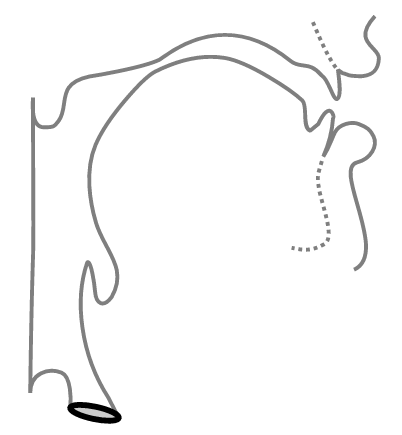
\includegraphics[width=0.2\linewidth]{02-i.png}}{1}
\putcvowel{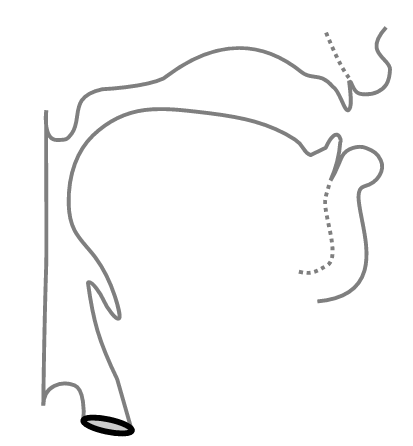
\includegraphics[width=0.2\linewidth]{03-a.png}}{4}
\putcvowel{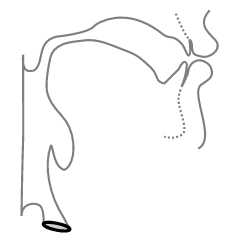
\includegraphics[width=0.2\linewidth]{04-u.png}}{8}
\end{vowel}
\end{center}
\vfill
\end{frame}

\begin{frame}{Как форма речевого аппарата влияет на гласные?}
\Large
\vfill
\begin{center}
\begin{vowel}
\putcvowel{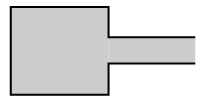
\includegraphics[width=0.2\linewidth]{05-i-tube.png}}{1}
\putcvowel{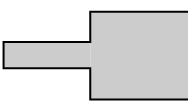
\includegraphics[width=0.2\linewidth]{06-a-tube.png}}{4}
\putcvowel{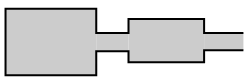
\includegraphics[width=0.2\linewidth]{07-u-tube.png}}{8}
\end{vowel}
\end{center}
\vfill
\end{frame}

\begin{frame}{Как форма речевого аппарата влияет на гласные?}
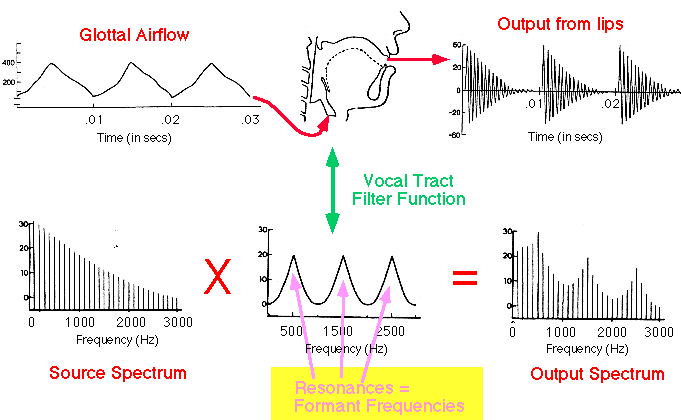
\includegraphics[width=0.95\linewidth]{01-source-filter.png}
\end{frame}

\begin{frame}{Как форма речевого аппарата влияет на гласные?}
\Large
\vfill
\begin{center}
\begin{vowel}
\putcvowel{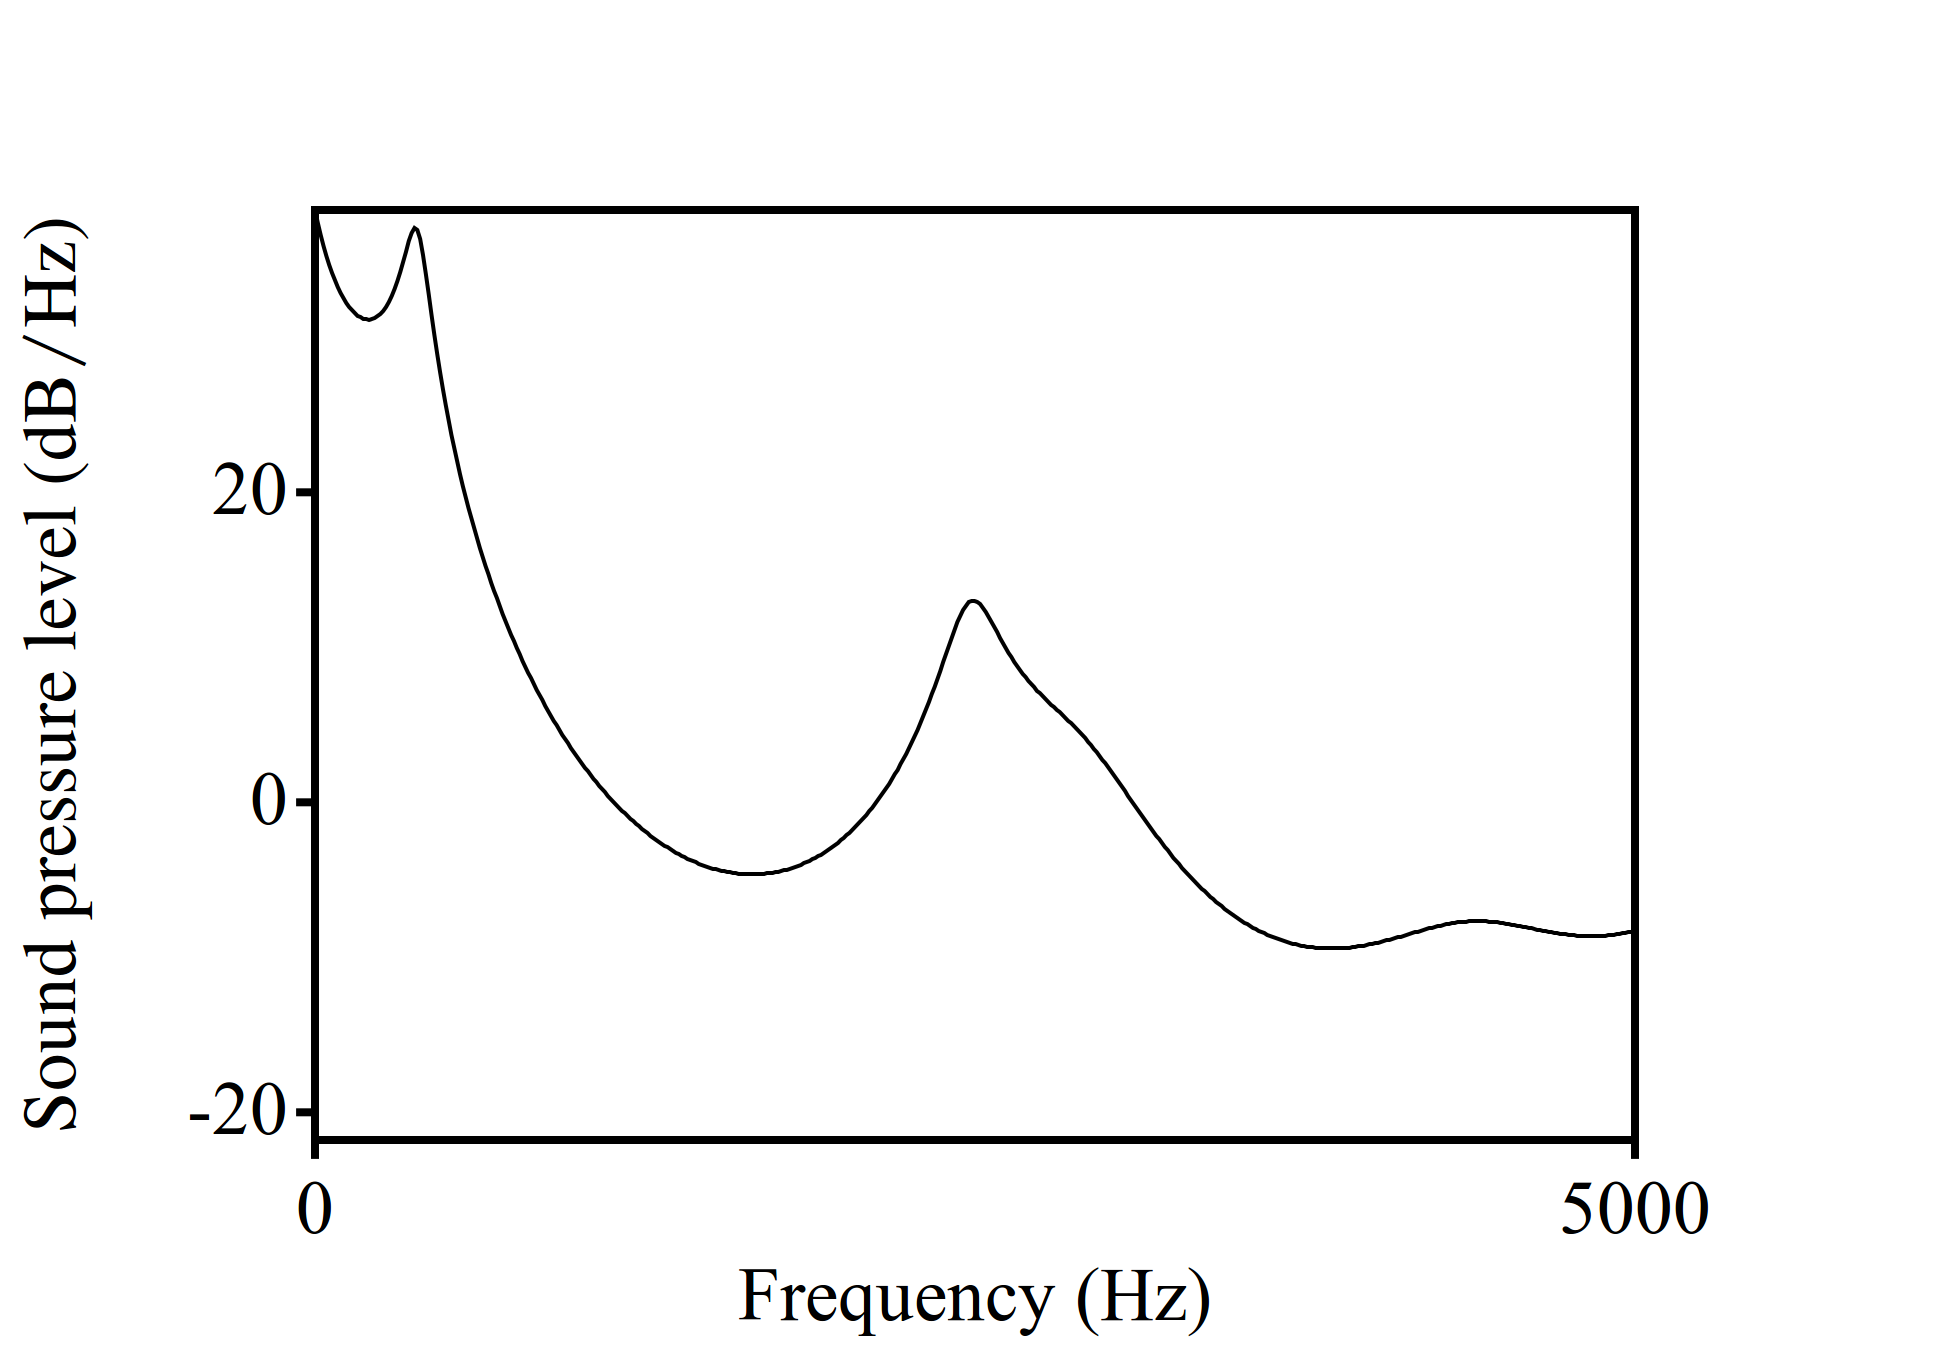
\includegraphics[width=0.3\linewidth]{08-i-spectrum.png}}{1}
\putcvowel{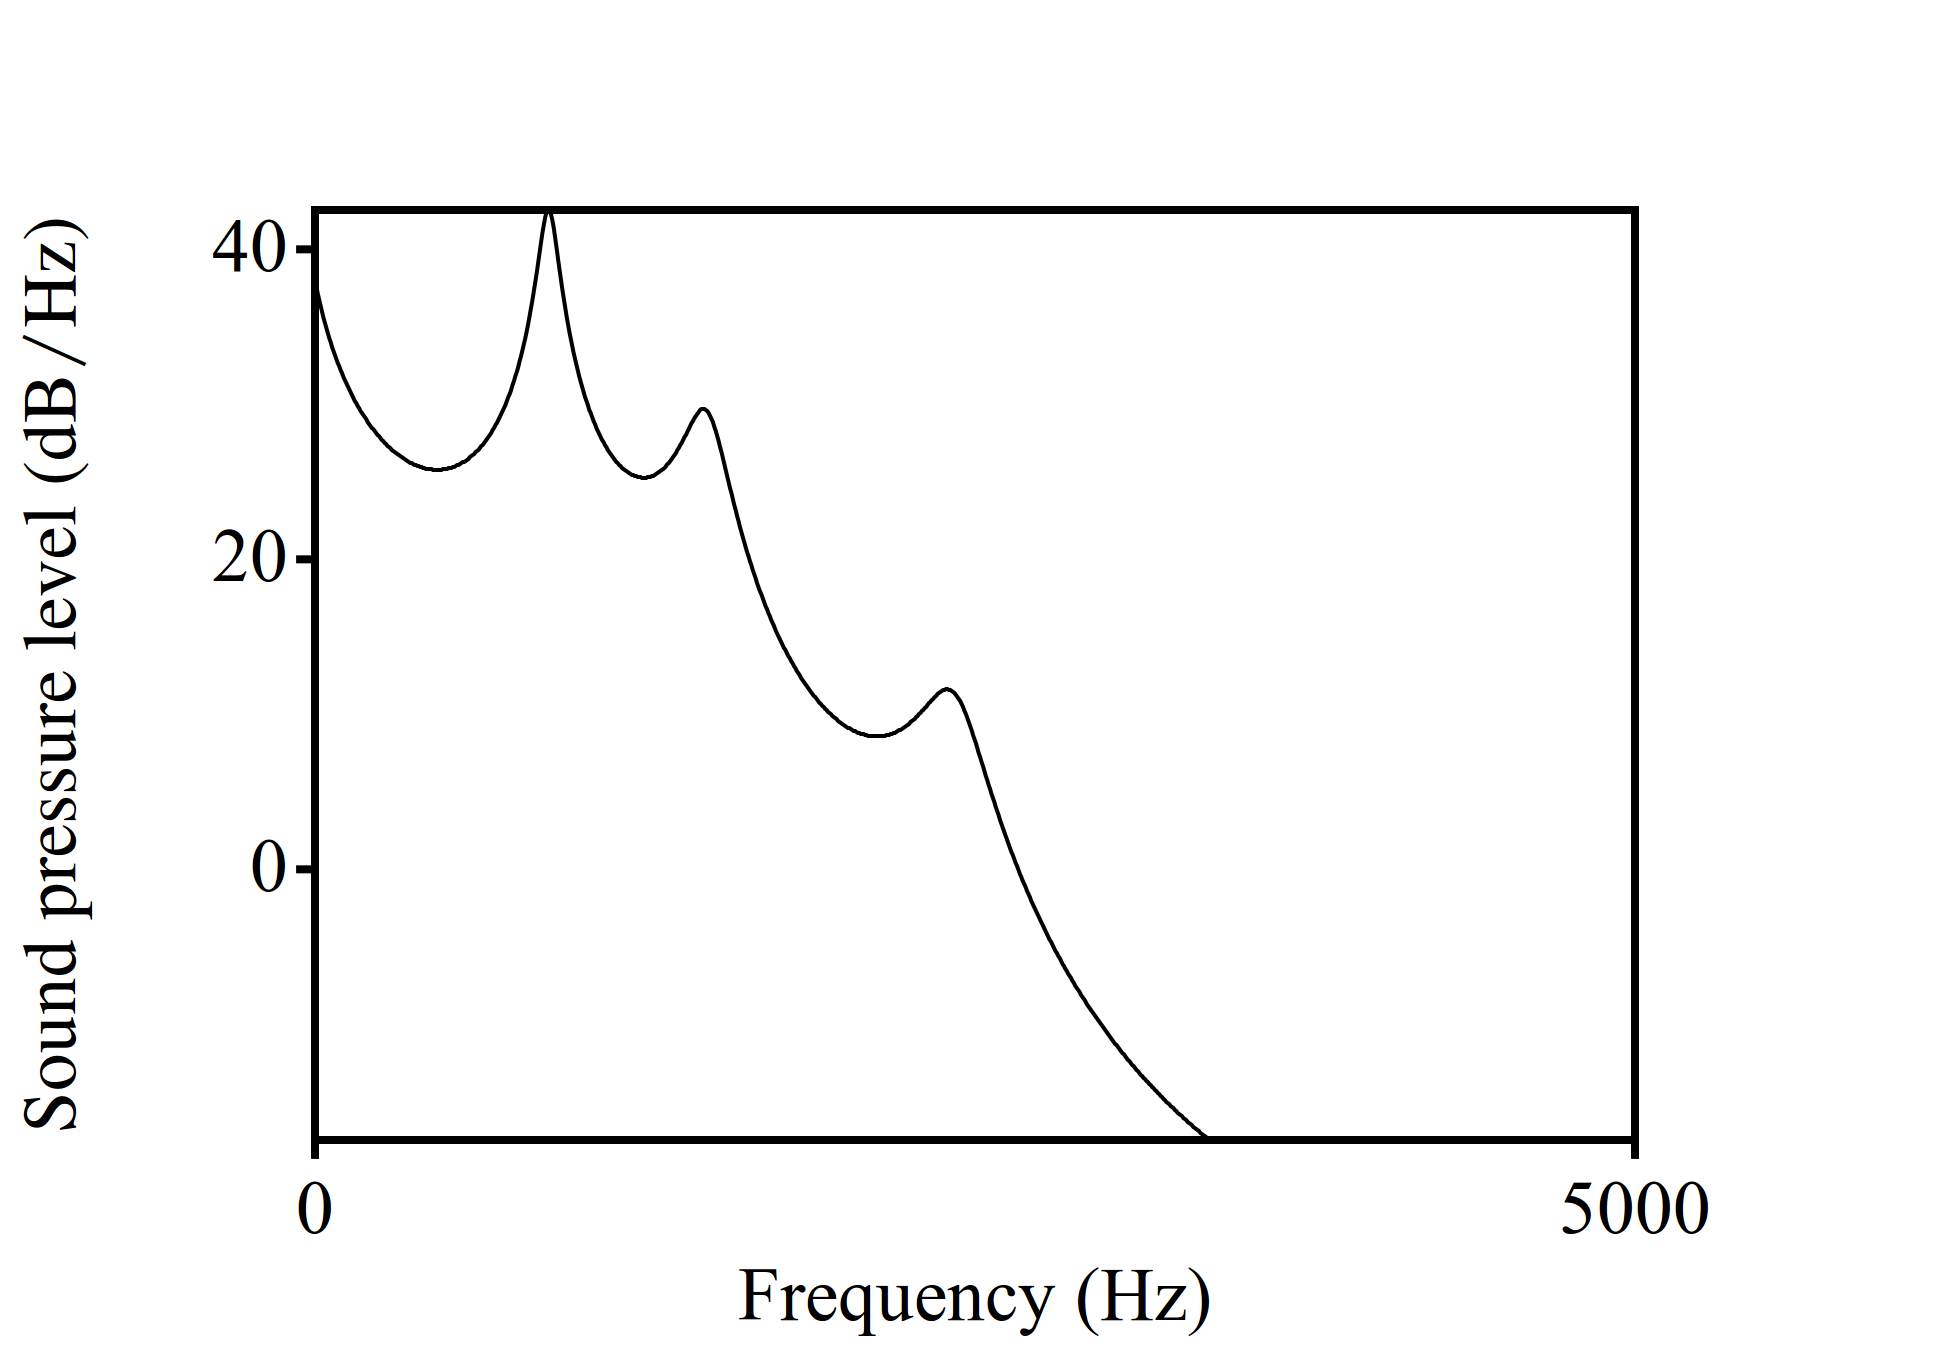
\includegraphics[width=0.3\linewidth]{09-a-spectrum.png}}{4}
\putcvowel{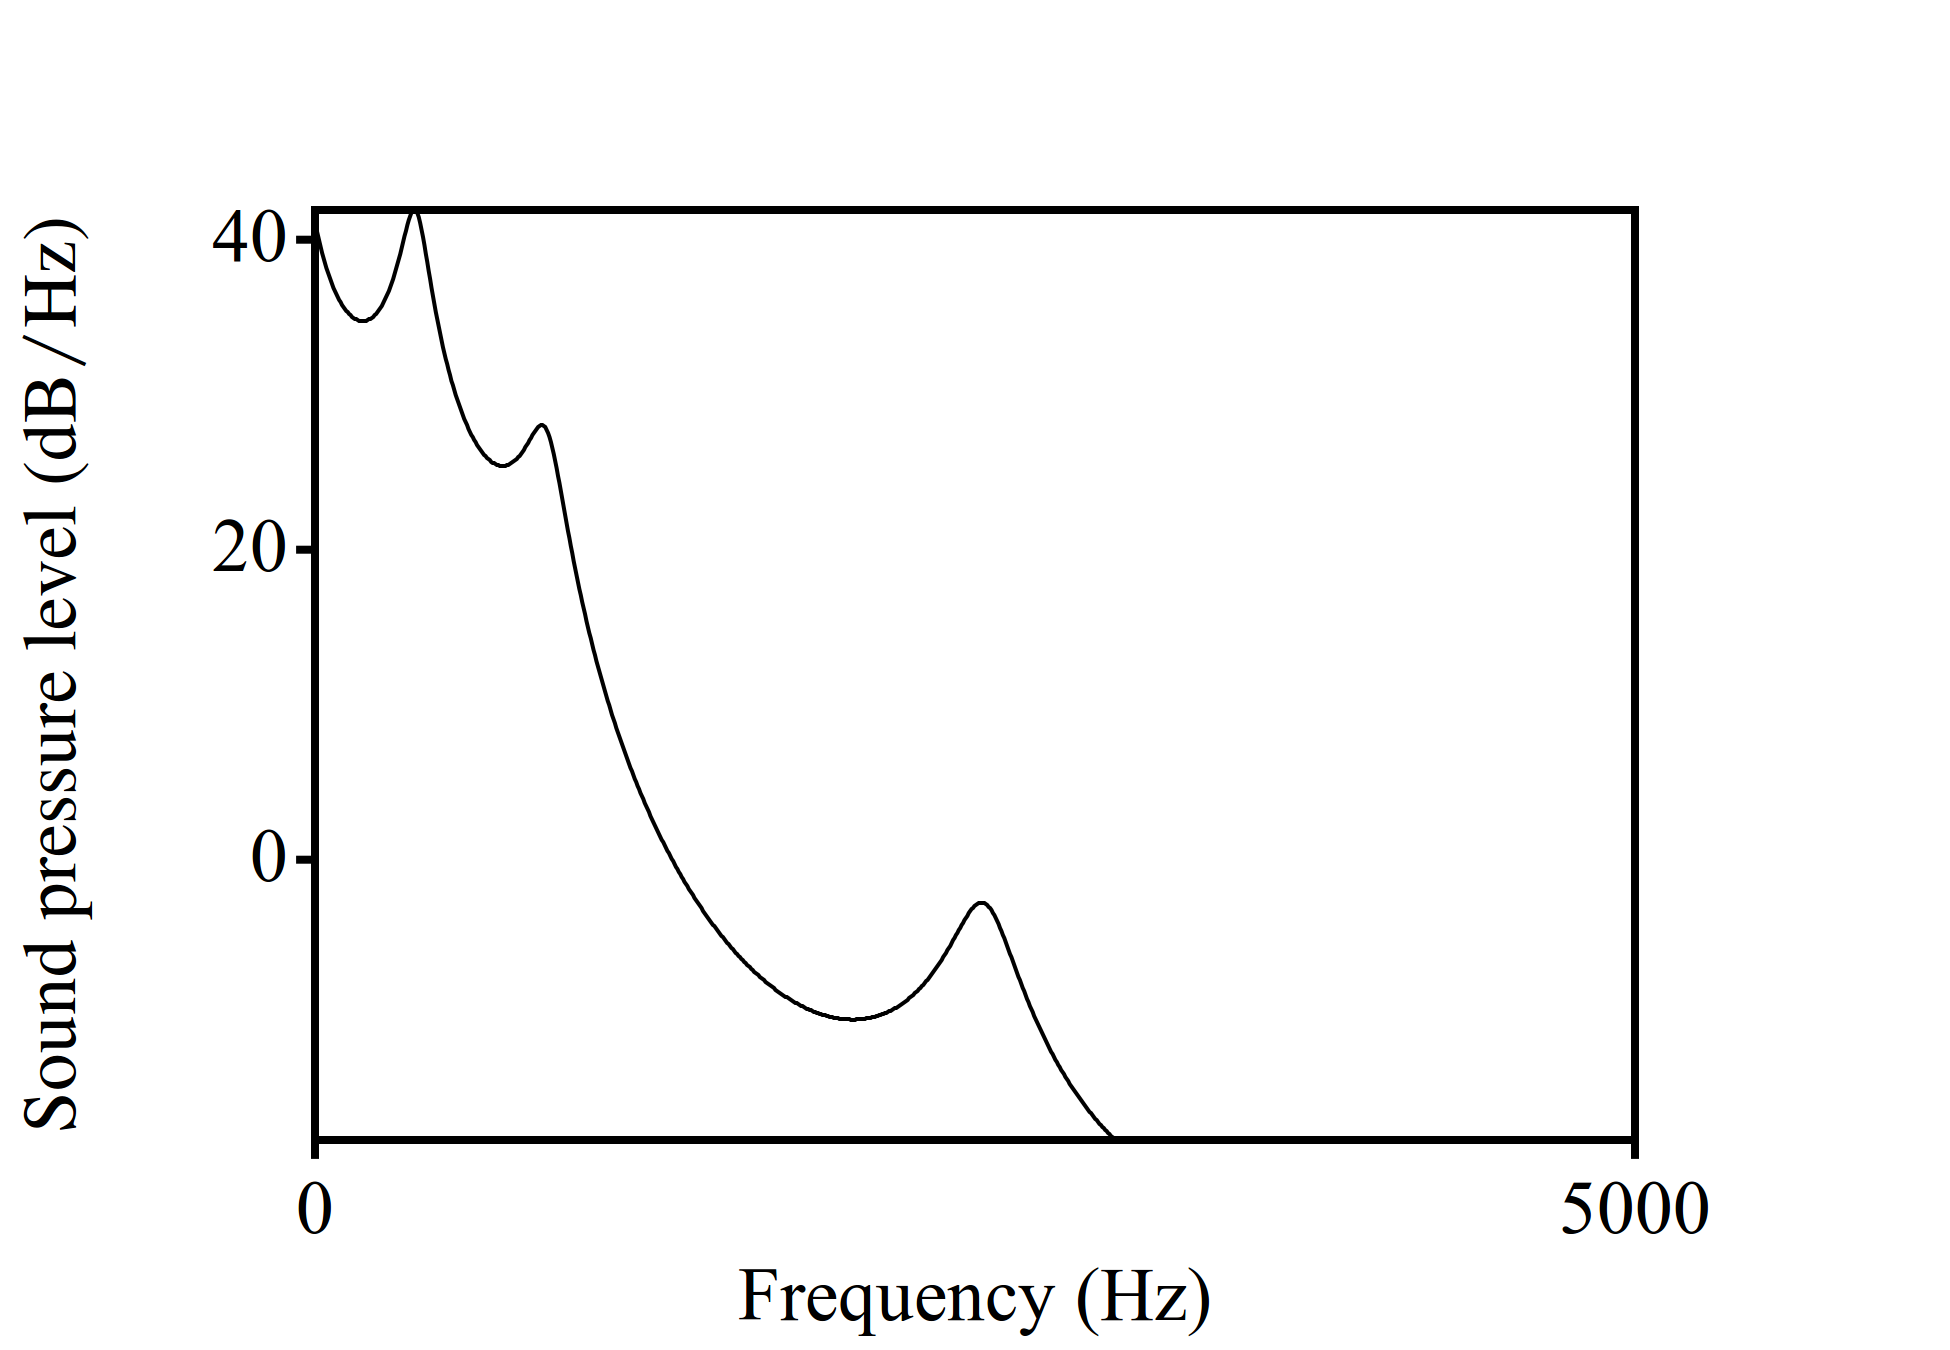
\includegraphics[width=0.3\linewidth]{10-u-spectrum.png}}{8}
\end{vowel}
\end{center}
\vfill
\end{frame}

\section{фонация}
\begin{frame}{Типы фонации}
Разные типы фонации --- результат \href{https://www.youtube.com/watch?v=b89RSYCaUBo}{работы гортани}.

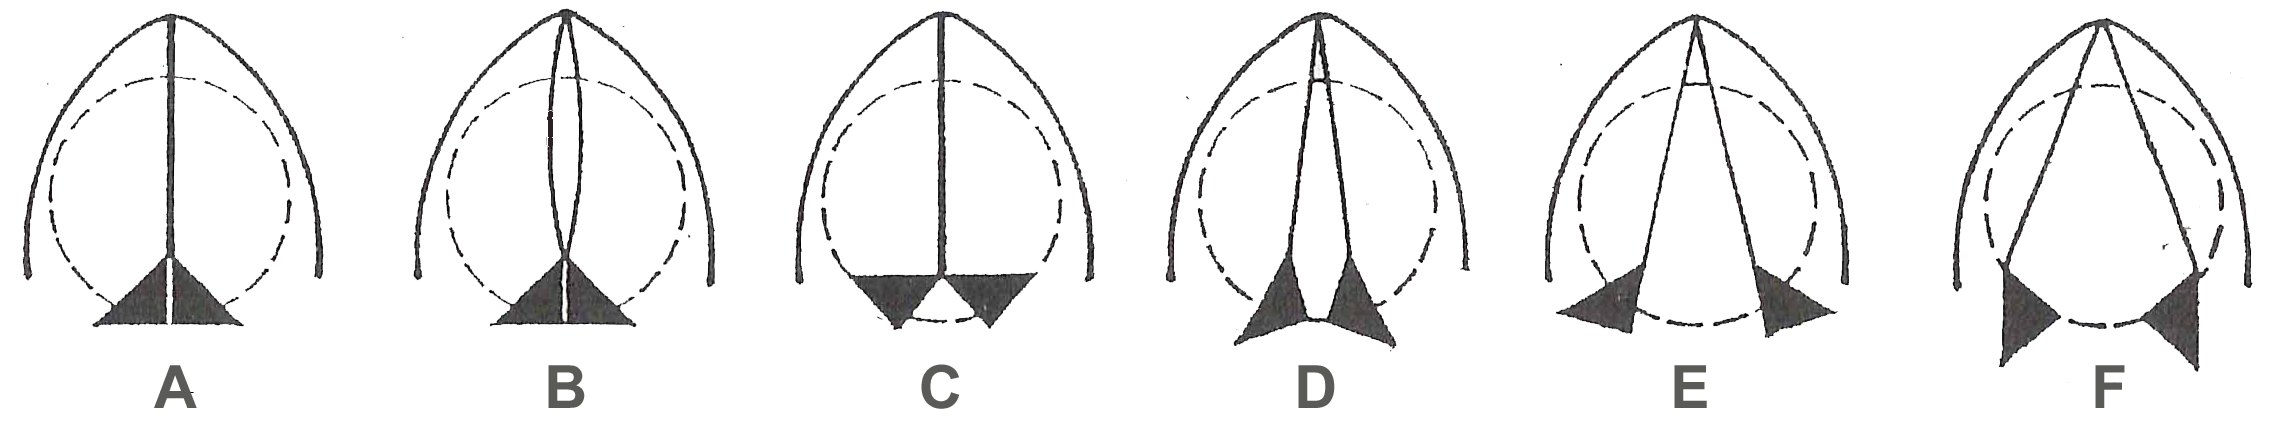
\includegraphics[width=\linewidth]{11-glottis-positions.png}

\begin{itemize}
\item[A] голосовые связки сомкнуты: \textbf{глотальный стоп, как в \textit{не-а}}
\item[B] воздух проходит через сомкнутые голосовые связки: \textbf{скрипучий голос}
\item[C]  воздух свободно проходит сквозь голосовые связки, заставляя их вибрировать \textbf{нейтральная фонация}
\item[D] поток воздуха проходит через голосовые связки, заставляя их незначительно колебаться (\textbf{придыхательная фонация})
\item[E]  голосвоые связки разведены \textbf{дыхание}
\item[F] голосовые связки достаточно сильно разведены \textbf{аспирация}
\end{itemize}
\end{frame}

\begin{frame}{Шумные согласные}
\begin{itemize}
\item взрывные: смычка - взрыв - время до гласного
\item фрикативные: турбулентный шум - гласный
\item аффрикаты: смычка - взрыв - турбулентный шум - гласный
\end{itemize}
\end{frame}

\section{}
\begin{frame}
{\huge Спасибо, что дослушали!\bigskip\\
agricolamz@gmail.com
\vspace{-130pt}}
\end{frame}
\end{document}
